\documentclass[11pt]{article}

% Change "review" to "final" to generate the final (sometimes called camera-ready) version.
% Change to "preprint" to generate a non-anonymous version with page numbers.
\usepackage[review]{acl}

% Standard package includes
\usepackage{times}
\usepackage{latexsym}

% For proper rendering and hyphenation of words containing Latin characters (including in bib files)
\usepackage[T1]{fontenc}
% For Vietnamese characters
% \usepackage[T5]{fontenc}
% See https://www.latex-project.org/help/documentation/encguide.pdf for other character sets

% This assumes your files are encoded as UTF8
\usepackage[utf8]{inputenc}

% This is not strictly necessary, and may be commented out,
% but it will improve the layout of the manuscript,
% and will typically save some space.
\usepackage{microtype}

% This is also not strictly necessary, and may be commented out.
% However, it will improve the aesthetics of text in
% the typewriter font.
\usepackage{inconsolata}

%Including images in your LaTeX document requires adding
%additional package(s)
\usepackage{graphicx}
\graphicspath{{../figs/}}

\usepackage{amsmath,amssymb}
\usepackage{booktabs}
\usepackage{multirow}
\usepackage[most]{tcolorbox}

% Shared math notation for the paper.
\newcommand{\R}{\mathbb{R}}
\newcommand{\E}{\mathbb{E}}
\newcommand{\Df}{\mathcal{D}_f}
\newcommand{\Dr}{\mathcal{D}_r}
\newcommand{\PPL}{\mathrm{PPL}}
\newcommand{\Lone}{L_1}
\newcommand{\Ltwo}{L_2}
\newcommand{\Lthree}{L_3}
\DeclareMathOperator*{\argmin}{arg\,min}
\DeclareMathOperator*{\argmax}{arg\,max}
\newcommand{\geomean}{\mathrm{geo}}

% If the title and author information does not fit in the area allocated, uncomment the following
%
%\setlength\titlebox{<dim>}
%
% and set <dim> to something 5cm or larger.

\title{From Three-Layer Unlearning Impact to Forget-Set Audit:\\
       Predicting Impact Profiles from Forget-Set Geometry Alone}

% Author information can be set in various styles:
% For several authors from the same institution:
% \author{Author 1 \and ... \and Author n \\
%         Address line \\ ... \\ Address line}
% if the names do not fit well on one line use
%         Author 1 \\ {\bf Author 2} \\ ... \\ {\bf Author n} \\
% For authors from different institutions:
% \author{Author 1 \\ Address line \\  ... \\ Address line
%         \And  ... \And
%         Author n \\ Address line \\ ... \\ Address line}
% To start a separate ``row'' of authors use \AND, as in
% \author{Author 1 \\ Address line \\  ... \\ Address line
%         \AND
%         Author 2 \\ Address line \\ ... \\ Address line \And
%         Author 3 \\ Address line \\ ... \\ Address line}

\author{First Author \\
  Affiliation / Address line 1 \\
  Affiliation / Address line 2 \\
  Affiliation / Address line 3 \\
  \texttt{email@domain} \\\And
  Second Author \\
  Affiliation / Address line 1 \\
  Affiliation / Address line 2 \\
  Affiliation / Address line 3 \\
  \texttt{email@domain} \\}

%\author{
%  \textbf{First Author\textsuperscript{1}},
%  \textbf{Second Author\textsuperscript{1,2}},
%  \textbf{Third T. Author\textsuperscript{1}},
%  \textbf{Fourth Author\textsuperscript{1}},
%\\
%  \textbf{Fifth Author\textsuperscript{1,2}},
%  \textbf{Sixth Author\textsuperscript{1}},
%  \textbf{Seventh Author\textsuperscript{1}},
%  \textbf{Eighth Author \textsuperscript{1,2,3,4}},
%\\
%  \textbf{Ninth Author\textsuperscript{1}},
%  \textbf{Tenth Author\textsuperscript{1}},
%  \textbf{Eleventh E. Author\textsuperscript{1,2,3,4,5}},
%  \textbf{Twelfth Author\textsuperscript{1}},
%\\
%  \textbf{Thirteenth Author\textsuperscript{3}},
%  \textbf{Fourteenth F. Author\textsuperscript{2,4}},
%  \textbf{Fifteenth Author\textsuperscript{1}},
%  \textbf{Sixteenth Author\textsuperscript{1}},
%\\
%  \textbf{Seventeenth S. Author\textsuperscript{4,5}},
%  \textbf{Eighteenth Author\textsuperscript{3,4}},
%  \textbf{Nineteenth N. Author\textsuperscript{2,5}},
%  \textbf{Twentieth Author\textsuperscript{1}}
%\\
%\\
%  \textsuperscript{1}Affiliation 1,
%  \textsuperscript{2}Affiliation 2,
%  \textsuperscript{3}Affiliation 3,
%  \textsuperscript{4}Affiliation 4,
%  \textsuperscript{5}Affiliation 5
%\\
%  \small{
%    \textbf{Correspondence:} \href{mailto:email@domain}{email@domain}
%  }
%}

\begin{document}
\maketitle
\begin{abstract}
      % Problem.
      Large language model (LLM) unlearning must remove target knowledge represented by a forget set $\Df$ while limiting collateral damage to useful knowledge.
      % Gap.
      Existing evaluations usually collapse this requirement into aggregate forget/retain scores or compare algorithms on a fixed forget split, leaving unclear how unlearning impact spreads from the target set to neighbouring and unrelated text, and whether damaging forget sets can be identified before running unlearning.
      % Method.
      We construct $100$ WikiText-103 triplets, unlearn Llama-3.1-8B-Instruct with GradAscent for each forget set, and evaluate all checkpoints against all triplets in a $100\times100$ cross-PPL matrix, yielding $1.5$M per-sample perplexity ratios.
      % Key mechanism.
      We represent each run by a \emph{three-layer impact profile}: intended degradation on $\Df$ ($\Lone$), neighbour impact on held-out same-triplet samples ($\Ltwo$), and bystander impact on off-diagonal test samples ($\Lthree$); we then predict this profile from a $12$-feature intrinsic geometry descriptor of $\Df$ using a leave-one-out Random Forest auditor.
      % Results.
      Impact decays across layers ($\Lone{=}1.96\times$, $\Ltwo{=}1.32\times$, $\Lthree{=}1.19\times$), but spillover does not vanish: $73.8\%$ of off-diagonal bystander samples have elevated PPL, and $\Lone$ varies by $1.59\times$ across forget sets under the same algorithm and hyperparameters. The geometry-only auditor gives rank-significant predictions for all layers (Spearman $\rho{=}0.56/0.87/0.59$ for $\Lone/\Ltwo/\Lthree$), and an independent NPO replication remains rank-significant ($\rho{=}0.66/0.82/0.51$, all CIs above zero).
      % Claim.
      Unlearning side effects are partly a property of the forget set itself, and forget-set geometry can provide a cheap pre-screen for risky candidates before full unlearning evaluation.
\end{abstract}

\section{Introduction}
\label{sec:intro}

% motivation
After deployment, large language models are increasingly asked to remove
specific knowledge. Copyright disputes, privacy regulation, user deletion
requests, and the discovery of toxic, private, or copyrighted content in
pretraining corpora all create cases where a model should stop reproducing or
relying on a target forget set $\Df$
\citep{maini2024tofu, shi2024muse, dorna2025openunlearning}. Since retraining
from scratch is usually impractical, \emph{LLM unlearning} aims to suppress
this target knowledge through post-training updates while preserving the rest
of the model. This preservation requirement is critical: in deployed systems, a
successful deletion is not sufficient if the same update silently corrupts
nearby facts, paraphrases, or unrelated capabilities.

% gap
Existing unlearning evaluations do not yet expose this side effect with enough
resolution. Most studies report aggregate utility or a small set of post-hoc
probes, which can miss the \emph{geometry} of unlearning damage: how impact
changes as evaluation text moves from the forget set itself, to same-topic
neighbours, to off-target bystanders. Recent knowledge-hole probing work
shows that benchmark-level utility can remain high even when adjacent or latent
knowledge is corrupted \citep{ko2025probing}. At the same time, most benchmarks
fix the forget split and compare algorithms, treating the choice of $\Df$ as
given. This leaves a practical question unanswered: among many candidate forget
sets, can we identify which ones are likely to cause broader damage before
running expensive unlearning?

\begin{tcolorbox}[
    colback=gray!10, colframe=gray!50,
    arc=2mm, boxrule=0.4pt,
    left=6pt, right=6pt, top=4pt, bottom=4pt,
]
\textbf{Research questions.}\\[2pt]
\textbf{RQ1.} Does collateral damage vary systematically with the choice of forget set?\\
\textbf{RQ2.} If yes, can it be predicted from forget-set geometry alone, before running unlearning?
\end{tcolorbox}

% method and insight
We address this question with a controlled cross-evaluation framework for
three-layer unlearning impact. We cluster WikiText-103 passages into semantic
groups, sample $100$ candidate triplets, and split each triplet into disjoint
train, validation, and test texts. For each triplet, the train split is the
forget set $\Df$, while validation and test texts provide held-out same-topic
neighbours. After unlearning Llama-3.1-8B-Instruct with a fixed GradAscent
configuration, we evaluate every unlearned checkpoint on every triplet,
yielding a cross-PPL matrix with $1.5$M per-sample perplexity ratios. This
matrix separates \textbf{intended degradation} on the forget set ($\Lone$),
\textbf{locality damage} on same-topic held-out text ($\Ltwo$), and
\textbf{spillover damage} on off-diagonal bystanders ($\Lthree$). The core
insight is that unlearning impact is structured by semantic distance, but the
chosen forget set also has an intrinsic geometry that helps predict how severe
that impact will be.

% results
Our measurements show both distance decay and persistent collateral damage.
Across the cross-PPL matrix, impact decreases strictly across the three layers
($\Lone{>}\Ltwo{>}\Lthree$), yet it does not vanish: $\Lthree$ remains above the
base model on $73.8\%$ of off-diagonal bystander samples. Damage magnitude also varies substantially with the chosen forget
set, even under the same algorithm and hyperparameters; $\Lone$ varies by
$1.59\times$ across the $100$ candidates. We then formulate \emph{forget-set
audit}: predicting the three-layer impact profile from forget-set geometry
alone. Using a $12$-dimensional intrinsic geometry descriptor computed from the
$50$ forget-set embeddings, a Random Forest regressor obtains rank-significant
predictions under leave-one-out cross-validation, with Spearman correlations of
$0.56$, $0.87$, and $0.59$ for $\Lone$, $\Ltwo$, and $\Lthree$; all $95\%$
bootstrap confidence intervals exclude zero. The auditor runs in seconds and
serves as a pre-screen for forget-set selection before full unlearning.

% contributions
Our contributions are:
(1) We introduce a measurement framework for three-layer unlearning impact,
separating intended forget-set degradation, same-topic locality damage, and
off-diagonal spillover damage within a unified cross-PPL matrix.
(2) We provide quantitative evidence that unlearning impact decays with
semantic distance, yet collateral damage remains non-zero even far from the
forget set: $\Lthree > 1$ on $73.8\%$ of off-diagonal bystander samples.
(3) We formulate \emph{forget-set audit}, which predicts the three-layer impact
profile from forget-set geometry alone. A $12$-feature Random Forest auditor
achieves rank-significant predictions across all three layers, including
$\rho = 0.87$ and $R^2 = 0.74$ for locality damage, enabling cheap screening
before full unlearning.

% roadmap
Sec.~\ref{sec:problem} formalises the three-layer impact and audit problems.
Sec.~\ref{sec:setup} describes the triplet schema, unlearning procedure, and
cross-PPL matrix. Sec.~\ref{sec:three-layer} reports the three-layer impact
findings. Sec.~\ref{sec:audit} presents the audit features, forget-set audit,
and predictor. Sec.~\ref{sec:discussion} discusses mechanisms, failure modes,
and practical considerations. Sec.~\ref{sec:conclusion} concludes, and
Sec.~\ref{sec:related}--\ref{sec:limitations} cover related work and
limitations.

% ============================================================================
% 2. Problem Formulation
% ============================================================================
\section{Problem Formulation}
\label{sec:problem}

% experimental object
\paragraph{Experimental objects.}
Let $M_{\theta_0}$ denote the original language model before unlearning, and
let $\mathcal{U}$ be a fixed post-training unlearning algorithm. We consider a
collection of candidate semantic groups
$\mathcal{G}=\{G_i\}_{i=1}^{N}$, where each group contains passages about a
coherent topic. Each group is split into three disjoint subsets:
$G_i^{\mathrm{tr}}$, $G_i^{\mathrm{val}}$, and $G_i^{\mathrm{te}}$. For
candidate $i$, the forget set and resulting unlearned checkpoint are
\begin{align}
    \Df^{(i)} &= G_i^{\mathrm{tr}},\\
    M_{\theta_i} &= \mathcal{U}(M_{\theta_0}, \Df^{(i)}).
\end{align}
The experiment fixes $M_{\theta_0}$ and $\mathcal{U}$, varies only
$\Df^{(i)}$, and compares the resulting checkpoints across the same semantic
groups.

% measurement metric
\paragraph{Measurement metric.}
For an evaluation passage $x$, we measure unlearning impact by the
base-normalised perplexity ratio
\begin{align}
    r_i(x)
    &=
    \frac{\PPL(M_{\theta_i}, x)}
         {\PPL(M_{\theta_0}, x)},\\
    R_i(S)
    &=
    \exp\!\left(
    \frac{1}{|S|}\sum_{x\in S}\log r_i(x)
    \right).
\end{align}
A value $r_i(x)>1$ means that unlearning $\Df^{(i)}$ makes the model assign
lower likelihood to $x$ than the original model did. For a set of passages
$S$, $R_i(S)$ is the geometric mean ratio. Normalising by $M_{\theta_0}$ makes
measurements comparable across
passages with different base difficulty.

% three-layer impact
\paragraph{Three-layer impact profile.}
For each candidate forget set $\Df^{(i)}$, we separate impact into three
semantic layers. Let
$\mathcal{N}^{(i)}=G_i^{\mathrm{val}}\cup G_i^{\mathrm{te}}$ be the held-out
same-triplet neighbour set, and let
$\mathcal{B}^{(i)}=\bigcup_{j\neq i}G_j^{\mathrm{te}}$ be the off-diagonal
bystander set. The three-layer impact profile is
\begin{align}
    \Lone^{(i)} &= R_i(G_i^{\mathrm{tr}})
    &&\text{(intended degradation)},\\
    \Ltwo^{(i)} &= R_i(\mathcal{N}^{(i)})
    &&\text{(locality damage)},\\
    \Lthree^{(i)} &= R_i(\mathcal{B}^{(i)})
    &&\text{(off-diagonal spillover)},\\
    \mathbf{y}^{(i)}
    &=\left(\Lone^{(i)},\Ltwo^{(i)},\Lthree^{(i)}\right).
\end{align}
High $\Lone$ is the intended forgetting signal; high $\Ltwo$ or $\Lthree$
indicates collateral damage.

% forget-set audit
\paragraph{Forget-set audit.}
Measuring $\mathbf{y}^{(i)}$ requires running $\mathcal{U}$ and evaluating the
resulting checkpoint. We formulate \emph{forget-set audit} as a
pre-unlearning prediction task: given only the candidate forget set
$\Df^{(i)}$, predict its future three-layer impact profile. Let
$\phi(\Df^{(i)})\in\R^d$ be an intrinsic descriptor computed from the
forget-set passages. An auditor
$A_{\psi}: \R^d \rightarrow \R^3$ is trained with the objective
\begin{equation}
    \hat{\psi}
    =
    \argmin_{\psi}
    \sum_{i=1}^{N}
    \left\|
    A_{\psi}\!\left(\phi(\Df^{(i)})\right)
    -
    \mathbf{y}^{(i)}
    \right\|_2^2.
\end{equation}
At prediction time, the auditor has no access to $M_{\theta_i}$ or to
post-unlearning evaluation results. Its practical goal is to estimate or rank
which candidate forget sets are likely to induce larger intended degradation,
same-topic locality damage, or off-diagonal spillover damage before paying for
full unlearning and cross-evaluation.

% ============================================================================
% 3. Experimental Setup
% ============================================================================
\section{Experimental Setup}
\label{sec:setup}

\subsection{Triplet Schema}
\label{sec:triplets}

We start from WikiText-103 \citep{merity2017pointer}, filter to $16{,}038$
usable passages, and embed them with \texttt{all-MiniLM-L6-v2}
\citep{wang2020minilmv2} into $384$-dimensional vectors. HDBSCAN
\citep{campello2013density} with \texttt{min\_cluster\_size}{=}$200$,
\texttt{min\_samples}{=}$5$, Euclidean distance, and Excess-of-Mass (EOM) cluster selection
produces $10$ non-noise semantic clusters and a noise pool of $9{,}198$
passages ($57.4\%$). We discard the noise pool and use only the clustered
passages when constructing forget-set candidates. Fig.~\ref{fig:triplet-schema}
summarises the construction.

\begin{center}
\centering
\setlength{\unitlength}{1pt}
\resizebox{0.98\columnwidth}{!}{%
\begin{picture}(240,310)
\footnotesize
\put(45,280){\framebox(150,24){\shortstack{WikiText-103\\raw passages}}}
\put(120,280){\vector(0,-1){14}}
\put(45,234){\framebox(150,32){\shortstack{Filter usable passages\\$16{,}038$ texts}}}
\put(120,234){\vector(0,-1){14}}
\put(45,188){\framebox(150,32){\shortstack{Embed passages\\MiniLM, $384$-d}}}
\put(120,188){\vector(0,-1){14}}
\put(45,142){\framebox(150,32){\shortstack{HDBSCAN clustering\\$10$ clusters + noise}}}
\put(120,142){\vector(0,-1){14}}
\put(45,96){\framebox(150,32){\shortstack{$10$ semantic clusters\\noise pool excluded}}}
\put(120,96){\vector(0,-1){14}}
\put(35,50){\framebox(170,32){\shortstack{Per cluster: sample $10$ triplets\\$100$ triplets total}}}
\put(120,50){\line(0,-1){8}}
\put(38,42){\line(1,0){164}}
\put(38,42){\vector(0,-1){8}}
\put(120,42){\vector(0,-1){8}}
\put(202,42){\vector(0,-1){8}}
\scriptsize
\put(0,0){\framebox(76,34){\shortstack{Forget set\\\texttt{train}\\$50$ texts}}}
\put(82,0){\framebox(76,34){\shortstack{Neighbour\\\texttt{val/test}\\same triplet}}}
\put(164,0){\framebox(76,34){\shortstack{Bystander\\other \texttt{test}\\off-diagonal}}}
\end{picture}}
\vspace{0.35em}
\refstepcounter{figure}\label{fig:triplet-schema}
\parbox{0.96\columnwidth}{\small\textbf{Figure~\thefigure:} Triplet schema. WikiText-103 passages are filtered, embedded, and clustered; each non-noise semantic cluster yields $10$ triplets. The train split is the forget set, validation/test splits are same-topic neighbours, and test splits from triplets in other clusters serve as cross-topic bystanders in off-diagonal evaluation.}
\end{center}

For each non-noise cluster we independently sample $10$ \emph{triplets}, giving
$100$ triplets in total. Each triplet contains three same-cluster but mutually
disjoint splits of $50$ texts:
\begin{center}
\small
\begin{tabular}{@{}ll@{}}
    \toprule
    Layer & Downstream role \\
    \midrule
    $\Lone$: forget set $\Df$ & unlearning target \\
    $\Ltwo$: neighbours       & neighbour knowledge \\
    $\Lthree$: bystanders     & unintended knowledge corruption \\
    \bottomrule
\end{tabular}
\end{center}
The within-triplet disjointness gives a clean separation between the unlearning
target, same-topic neighbour knowledge, and off-diagonal corruption probes. Triplets are sampled independently, so
two triplets drawn from the same cluster may reuse passages; triplets from
different clusters are disjoint by construction because HDBSCAN assigns each
passage to a single cluster. In the cross-PPL matrix, the matched validation
and test splits instantiate $\Ltwo$, while off-diagonal test splits instantiate
$\Lthree$.

\subsection{Unlearning Procedure}
\label{sec:unlearn}

We unlearn Llama-3.1-8B-Instruct \citep{dubey2024llama3} with the GradAscent objective \citep{jang2023knowledge}: for each $\Df$ we maximise the negative log-likelihood on $\Df$ while keeping a small retain-loss term on the same-cluster validation split. Hyperparameters follow defaults from OpenUnlearning \citep{dorna2025openunlearning}: learning rate $1\!\times\!10^{-5}$ with linear decay, paged AdamW (32-bit), per-device batch size $8$ with gradient accumulation $8$ (effective batch $64$), $5$ epochs (resulting in $5$ optimiser steps because $|\Df|{=}50<64$), warmup of $1$ step, weight decay $0.01$, BF16. All runs use a single H100 80\,GB. Each unlearn run takes $\approx 75$\,s wall-clock; the full $n{=}100$ sweep finishes in $1$\,h\,$54$\,min and produces $\approx 1.5$\,TB of checkpoints ($\approx 15$\,GB each). Train loss converges in $[-0.84, -0.62]$ (negative is expected for GradAscent).

\subsection{Cross-PPL Evaluation Protocol}
\label{sec:matrix}

To attribute observed spread cleanly to $\Df^{(i)}$, every unlearned checkpoint
$M_{\theta_i}$ is evaluated on the \emph{same} grid of $100$ triplets $\times\,3$
splits $\times\,50$ texts ($100 \times 100 \times 3 \times 50 = 1{.}5$M
per-sample ratios), rather than each checkpoint choosing its own bystander pool. This unified probe set ensures that differences in
$(\Lone^{(i)},\Ltwo^{(i)},\Lthree^{(i)})$ across $i$ cannot be attributed to
differences in the evaluation texts. Per-sample PPLs are normalised by the
matching base-model PPL (Sec.~\ref{sec:problem}), so absolute-difficulty
variation across passages cancels and ratios are comparable across the
$1.5$M-row pool. We aggregate ratios per layer by geometric mean and by the
fraction of samples with $r{>}1.1$. Base-model PPLs are cached once on the
$100\times3$ probe set; the full unlearned sweep takes $\approx 6$\,h\,$11$\,min
on one H100 ($\approx 2.2$\,s per checkpoint--triplet pair), and is exported as
a long-format table for downstream auditing.

% ============================================================================
% 4. Three-Layer Unlearning Impact
% ============================================================================
\section{Three-Layer Unlearning Impact}
\label{sec:three-layer}

This section reports the main empirical shape of unlearning impact. Following
Sec.~\ref{sec:problem}, we separate the effect of a single unlearning run into
three layers: $\Lone$ is the intended degradation on the forget set,
$\Ltwo$ is the impact on held-out same-topic neighbours, and $\Lthree$ is the
impact on cross-topic bystanders. Table~\ref{tab:headline} reports geometric
means of the per-sample PPL ratio $r$ across the $1.5$M evaluations, and
Fig.~\ref{fig:three-layer-decay} visualises the same pattern.

\begin{table}[t]
\centering
\small
\setlength{\tabcolsep}{4pt}
\begin{tabular}{@{}lccc@{}}
    \toprule
                                                   & $\Lone$ & $\Ltwo$ & $\Lthree$ \\
    \midrule
    Samples                                        & $5{,}000$ & $10{,}000$ & $495{,}000$ \\
    Geo-mean $r$                                   & \textbf{$1.96\times$} & \textbf{$1.32\times$} & \textbf{$1.19\times$} \\
    \% samples with $r{>}1.1$                      & $100.0$ & $90.8$ & $73.8$ \\
    \% samples with $r{>}2.0$                      & $42.0$  & $2.4$  & $0.8$ \\
    \bottomrule
\end{tabular}
\caption{Three-layer unlearning impact headline ($n{=}100$ forget sets, $1.5$M per-sample ratios). Impact decays strictly ($\Lone{>}\Ltwo{>}\Lthree$), but bystander impact remains measurable: $\Lthree{>}1$ on $73.8\%$ of cross-topic samples.}
\label{tab:headline}
\end{table}

\begin{figure}[t]
\centering
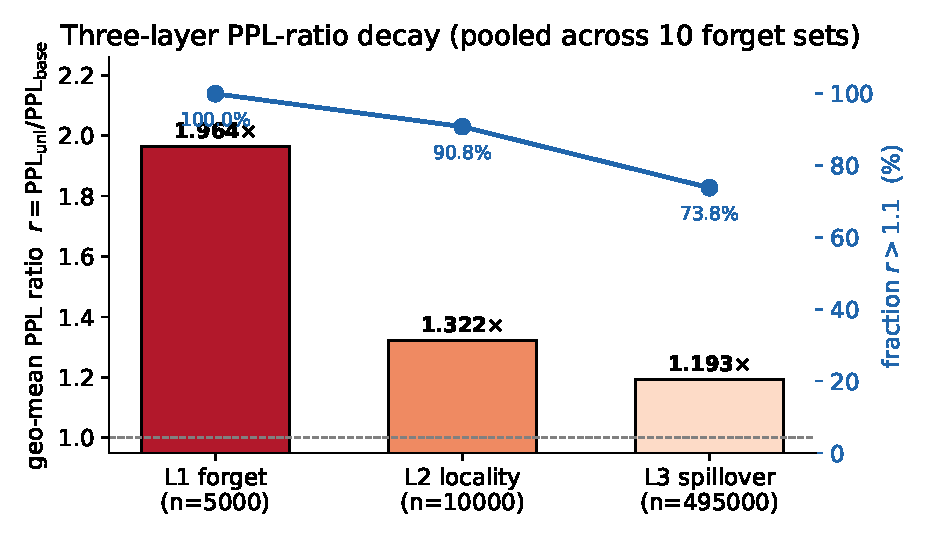
\includegraphics[width=0.95\columnwidth]{fig_three_layer_decay.pdf}
\caption{\textbf{Three-layer impact decay.} Left: geo-mean PPL ratio $r$ falls from $\Lone{=}1.96\times$ to $\Lthree{=}1.19\times$. Right: fraction of samples with $r{>}1.1$ ($100\%/90.8\%/73.8\%$). $\Lthree$ bystander impact is non-zero in both senses.}
\label{fig:three-layer-decay}
\end{figure}

We also examine whether the profile is fixed by the algorithm, or whether it
depends on which forget set is chosen. Under identical optimisation, switching
$\Df$ changes the measured profile substantially: Table~\ref{tab:perforget}
contrasts the mildest and worst forget set among $100$, and
Fig.~\ref{fig:per-forget-profile} shows the full distribution.

\begin{table}[t]
\centering
\small
\setlength{\tabcolsep}{4pt}
\begin{tabular}{@{}lccc@{}}
    \toprule
                                                   & $\Lone$ & $\Ltwo$ & $\Lthree$ \\
    \midrule
    Mildest triplet (\texttt{029})                 & $1.54$ & $1.15$ & $1.12$ \\
    Worst triplet (\texttt{073}, ``storm'')        & $\mathbf{2.44}$ & $\mathbf{1.73}$ & $\mathbf{1.26}$ \\
    \midrule
    Spread (max/min, $n{=}100$)                    & $\mathbf{1.59\times}$ & $1.50\times$ & $1.13\times$ \\
    \bottomrule
\end{tabular}
\caption{Forget-set-induced variation. $\Lone$ varies by $1.59\times$ between the mildest and worst $\Df$ under fixed algorithm/hyperparameters.}
\label{tab:perforget}
\end{table}

\begin{figure}[t]
\centering

\includegraphics[width=0.95\columnwidth]{fig_per_forget_profile.pdf}
\caption{\textbf{Per-forget-set variance ($n{=}100$).} Box + jitter of geo-mean $r$ for each layer; one dot per forget set. Spread $\max/\min$ reaches $1.59\times$ on $\Lone$, $1.50\times$ on $\Ltwo$, $1.13\times$ on $\Lthree$. \texttt{triplet\_073} (``storm'') is the worst on $\Lone$ and $\Ltwo$ but not on $\Lthree$ (where \texttt{triplet\_072} is the maximum, $1.26\times$); \texttt{triplet\_029} is the $\Lone$ minimum. Distribution shape is markedly tighter as the layer recedes from $\Df$.}
\label{fig:per-forget-profile}
\end{figure}

Together, these results support three observations.

\textbf{(C1) The three layers are strictly decreasing.}
The layer ordering is not an arbitrary binning choice: the measured impact
decreases monotonically from the forget set to neighbours to bystanders.
Table~\ref{tab:headline} gives
$\Lone{=}1.96\times{>}\Ltwo{=}1.32\times{>}\Lthree{=}1.19\times$, and
Fig.~\ref{fig:three-layer-decay} shows the same decay in both geo-mean PPL
ratio and the fraction of samples with $r{>}1.1$. The ordering also holds
within each cluster (Appendix~\ref{app:tables}), so it is not an artefact of
global aggregation.

\textbf{(C2) Bystander impact is not zero.}
The third layer is weaker than the first two, but cross-topic bystanders are
still measurably hit. $\Lthree$ has geo-mean $1.19\times$, and $73.8\%$ of
cross-topic samples exceed $r{>}1.1$. These samples are not in the forget set
and are not same-topic neighbours of the unlearned triplet, so this is genuine
spillover rather than intended forgetting.

\textbf{(C3) The profile varies with the forget set.}
The same algorithm and hyperparameters do not produce a single fixed impact
profile. In Table~\ref{tab:perforget}, changing only $\Df$ moves $\Lone$
from $1.54\times$ to $2.44\times$ and $\Ltwo$ from $1.15\times$ to
$1.73\times$; Fig.~\ref{fig:per-forget-profile} shows that this is a
distributional pattern rather than a single outlier. This variation makes the
forget set itself worth auditing before paying for full unlearning and
cross-evaluation.

% ============================================================================
% 5. Forget-Set Audit
% ============================================================================
\section{Forget-Set Audit}
\label{sec:audit}

Because the three-layer profile varies with $\Df$, forget-set choice becomes a
tunable design decision. The problem is that \emph{evaluating} that decision
currently requires running unlearning. We now ask whether $\Df$'s intrinsic
geometry is a sufficient signal to predict the three-layer impact profile
without ever fine-tuning.

\subsection{Audit Features}
\label{sec:features}

For each forget set $\Df$ of $50$ texts, we compute a $12$-dim intrinsic
geometric descriptor from the same MiniLM embeddings used for clustering, with
no access to model weights, gradients, or any unlearned checkpoint. The features
fall into four groups:
\begin{center}
\footnotesize
\begin{tabular}{@{}ll@{}}
    \toprule
    Group & Feature \\
    \midrule
    Spread (3)
        & \texttt{emb\_variance\_mean} \\
        & \texttt{emb\_variance\_max} \\
        & \texttt{pairwise\_eucl\_mean} \\
    Similarity (3)
        & \texttt{pairwise\_sim\_mean} \\
        & \texttt{pairwise\_sim\_std} \\
        & \texttt{pairwise\_sim\_q90} \\
    Location/scale (3)
        & \texttt{centroid\_norm} \\
        & \texttt{emb\_norm\_mean} \\
        & \texttt{emb\_norm\_std} \\
    Shape (3)
        & \texttt{effective\_rank} \\
        & \texttt{isotropy} \\
        & \texttt{spread\_over\_centroid} \\
    \bottomrule
\end{tabular}
\end{center}
All $12$ features are scalars derived from the $50\times 384$ forget-set embedding matrix; computing them takes milliseconds per $\Df$.

\subsection{Audit Problem}
\label{sec:audit-problem}

\paragraph{Input.} For a candidate forget set $\Df$, the auditor observes only
the embedding-derived feature vector $\phi(\Df)\in\mathbb{R}^{12}$ from
Sec.~\ref{sec:features}. It does not use an unlearned checkpoint, evaluation
texts, retain texts, gradients, or model weights.

\paragraph{Target.} The output is a three-dimensional prediction for the
future impact profile: geo-mean $\log r$ on $\Lone$, $\Ltwo$, and $\Lthree$.
Equivalently, exponentiating each coordinate gives the predicted layer-level
PPL ratio. We evaluate the auditor under two complementary task views:
(i) \emph{regression} (numeric fit) --- how close the predicted geo-mean $\log r$
is to the true value, scored by held-out $R^2$ and MAE against the LOO-mean
baseline; and (ii) \emph{ranking} --- whether the auditor correctly orders the
$100$ candidate forget sets by their future damage on each layer, scored by
Spearman $\rho$ with bootstrap CIs. Regression is the underlying learning
objective; ranking is the practical use case (pre-screen the riskiest $\Df$).

\paragraph{Training protocol.} We train one Random Forest regressor per layer
($n_{\text{est}}{=}200$, minimum leaf size $2$, unbounded depth, seed $0$).
Evaluation is leave-one-out over the $n{=}100$ forget sets: for each held-out
candidate, the auditor is fit on the other $99$ candidates and then predicts
the held-out impact profile. The baseline predicts the mean target value from
the $99$ training candidates. Ridge, Lasso, and Gradient Boosting variants use
the same features and LOO protocol and are reported in Sec.~\ref{sec:ablation}.

\subsection{Audit Performance}
\label{sec:audit-perf}

Table~\ref{tab:audit} reports held-out $R^2$, MAE, and Spearman $\rho$, plus $95\%$ percentile bootstrap CIs for $\rho$ ($n_{\text{boot}}{=}10{,}000$, seed $0$, bootstrapping over the $10$ LOO (true, predicted) cluster pairs).

\begin{table}[t]
\centering
\footnotesize
\setlength{\tabcolsep}{2.2pt}
\begin{tabular}{@{}lccc@{}}
    \toprule
                         & $\Lone$            & $\Ltwo$            & $\Lthree$            \\
    \midrule
    Audit $R^2$          & $\mathbf{+0.301}$  & $\mathbf{+0.735}$  & $\mathbf{+0.305}$    \\
    Mean $R^2$           & $-0.020$           & $-0.020$           & $-0.020$             \\
    Audit MAE            & $\mathbf{0.133}$   & $\mathbf{0.046}$   & $\mathbf{0.019}$     \\
    Mean MAE             & $0.169$            & $0.105$            & $0.022$              \\
    \midrule
    Spearman $\rho$      & $+0.560$           & $+0.869$           & $+0.592$             \\
    $\rho$ 95\% CI       & $[.40,.69]$        & $[.81,.91]$        & $[.44,.71]$          \\
    \bottomrule
\end{tabular}
\caption{Forget-set audit performance. LOO over $n{=}100$ forget sets; Random Forest ($n_{\text{est}}{=}200$, $\text{min\_leaf}{=}2$) on $12$-dim forget-set geometry. Mean rows are LOO mean baselines. All three $\rho$ CIs exclude zero; $\Ltwo$ is the strongest layer, and $\Lthree$ CI is now strictly above zero.}
\label{tab:audit}
\end{table}

\begin{figure*}[t]
\centering

\includegraphics[width=0.78\textwidth]{fig_audit_scatter.pdf}
\caption{\textbf{Audit scatter}, predicted vs.\ true geo-mean $\log r$. Each point is one held-out forget set under LOO. $\Ltwo$ is closest to the diagonal ($\rho{=}0.87$); $\Lone$ and $\Lthree$ are noisier but rank-significant ($\rho{=}0.56$, $0.59$).}
\label{fig:audit-scatter}
\end{figure*}

\begin{figure*}[t]
\centering
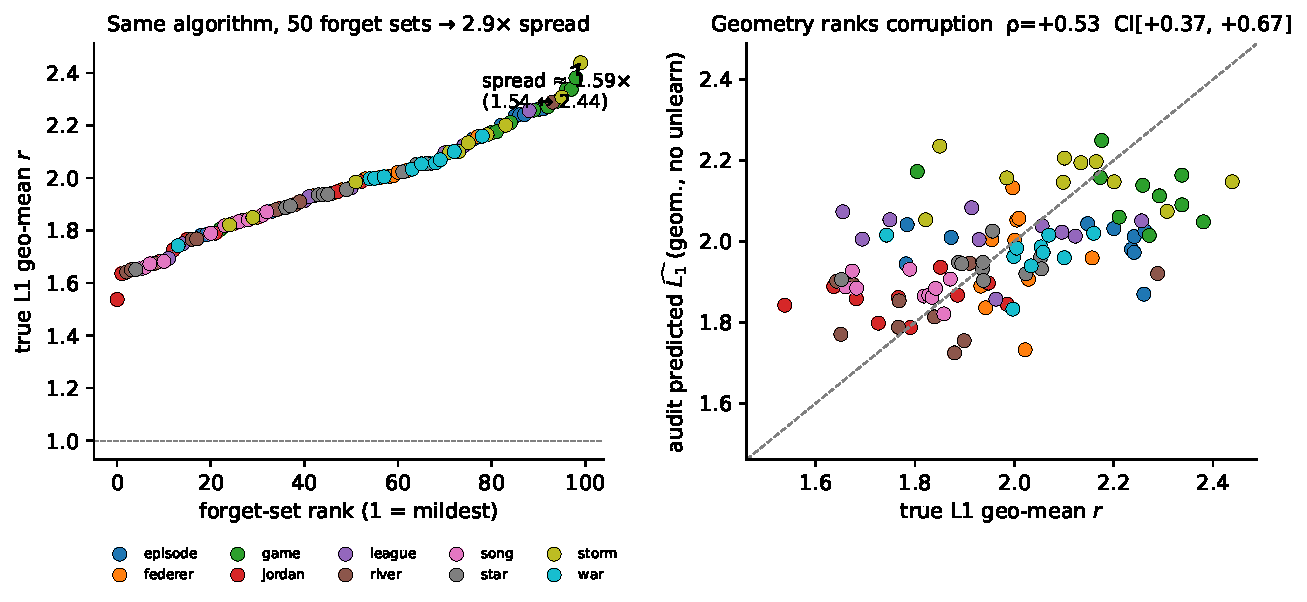
\includegraphics[width=0.78\textwidth]{fig_forget_spread.pdf}
\caption{\textbf{Forget-set spread.} Distribution of per-forget-set $\Lone$ across the $100$ triplets, grouped by HDBSCAN cluster. The variation auditing must capture is between-cluster more than within-cluster.}
\label{fig:forget-spread}
\end{figure*}

\textbf{$\Ltwo$ is the strongest layer.} With $R^2{=}0.74$ and $\rho{=}0.87$, the auditor recovers $74\%$ of locality variance from forget-set geometry alone --- consistent with the intuition that locality damage tracks how concentrated and self-similar $\Df$ is in embedding space.

\textbf{$\Lthree$ CI now excludes zero.} On a coarser problem ($n{=}10$ in early experiments) the L3 audit had $R^2{=}-0.46$; at $n{=}100$ the Random Forest auditor reaches $R^2{=}+0.30$ with $\rho{=}0.59$ ($95\%$ CI $[+0.44, +0.71]$). Statistical power and a non-linear model together close the previous gap; even the linear Ridge baseline (Sec.~\ref{sec:ablation}) reaches $\rho{=}0.49$ on the same $n{=}100$ slice.

\textbf{Audit cost.} Computing the $12$-dim feature for one $\Df$ takes milliseconds; fitting the Random Forest on $99$ training triplets is well under a second; predicting on a new $\Df$ is essentially instant. By contrast, evaluating one candidate $\Df$ via the standard pipeline costs one unlearn run ($\approx 75$\,s on H100) plus one column of cross-PPL ($\approx 220$\,s for $100$ eval pairs). At $n{=}100$ candidates the full grid is $\approx 7$ GPU-hours; the auditor runs in seconds on a CPU.

\subsection{Predictor Ablation}
\label{sec:ablation}

We compare the headline Random Forest auditor against three alternative
regressors on the same $12$-dim feature matrix and same LOO protocol
(Table~\ref{tab:ablation}): Ridge ($\alpha{=}1$, the simplest linear
baseline), Lasso ($\alpha{=}0.01$), and Gradient Boosting ($n_{\text{est}}{=}200$, $\text{depth}{=}3$, $\text{lr}{=}0.05$).

\begin{table}[t]
\centering
\small
\setlength{\tabcolsep}{3.5pt}
\begin{tabular}{@{}lccc@{}}
    \toprule
    Predictor                                 & $\Lone$            & $\Ltwo$            & $\Lthree$            \\
    \midrule
    \multicolumn{4}{@{}l@{}}{\textit{$R^2$ (LOO held-out)}} \\
    Random Forest (headline)                  & $\mathbf{+0.301}$  & $\mathbf{+0.735}$  & $\mathbf{+0.305}$    \\
    Gradient Boosting                         & $+0.209$           & $+0.743$           & $+0.200$             \\
    Ridge ($\alpha{=}1$)                      & $+0.246$           & $+0.705$           & $+0.215$             \\
    Lasso ($\alpha{=}0.01$)                   & $+0.224$           & $+0.644$           & $+0.088$             \\
    \midrule
    \multicolumn{4}{@{}l@{}}{\textit{Spearman $\rho$}} \\
    Random Forest (headline)                  & $\mathbf{+0.560}$  & $\mathbf{+0.869}$  & $\mathbf{+0.592}$    \\
    Gradient Boosting                         & $+0.524$           & $+0.879$           & $+0.534$             \\
    Ridge ($\alpha{=}1$)                      & $+0.531$           & $+0.840$           & $+0.491$             \\
    Lasso ($\alpha{=}0.01$)                   & $+0.494$           & $+0.849$           & $+0.380$             \\
    \bottomrule
\end{tabular}
\caption{Predictor ablation on the same $12$-dim feature matrix and LOO protocol ($n{=}100$). RF and GB are the strongest non-linear models and tie on $\Ltwo$; the linear Ridge baseline already lifts all three layers above the LOO-mean baseline ($R^2{=}{-}0.02$). Lasso under-fits on $\Lthree$ (sparse solution discards most features). Choosing the non-linear ceiling matters most for $\Lthree$, where RF gains $+0.09$ in $R^2$ over Ridge.}
\label{tab:ablation}
\end{table}

The non-linear models (RF, GB) tie on the strongest layer ($\Ltwo$), but RF
edges out on $\Lone$ and $\Lthree$ where forget-set geometry interactions
appear to matter more. The linear Ridge baseline ($\rho{=}0.49$ on $\Lthree$
with CI $[+0.33, +0.63]$, also strictly above zero) already gives a
deployable pre-screen, indicating that a substantial fraction of the
audit signal is linear in the geometric descriptor.

\subsection{Unlearner Generality (NPO)}
\label{sec:cross-unlearner}

To probe whether the audit framework is bound to GradAscent, we replicate the
full pipeline with NPO \citep{zhang2024negative}: a different unlearning
algorithm with the same TOFU-aligned hyperparameters on the same $n{=}100$
forget sets, yielding a parallel $100\times100$ cross-PPL grid and the same
$12$-dim geometric descriptor as input. The audit predictor (Random Forest,
identical hyperparameters and LOO protocol) is trained and evaluated
independently on NPO labels — we do not transfer predictions across unlearners.

\begin{table}[t]
\centering
\footnotesize
\setlength{\tabcolsep}{2.1pt}
\begin{tabular}{@{}llccc@{}}
    \toprule
    Metric & Alg. & $\Lone$ & $\Ltwo$ & $\Lthree$ \\
    \midrule
    geo $r$
       & GradAscent & $1.96\times$       & $1.32\times$       & $1.19\times$       \\
    geo $r$
       & NPO        & $1.68\times$       & $1.15\times$       & $1.11\times$       \\
    \midrule
    $\rho$
       & GradAscent & $+0.560$           & $\mathbf{+0.869}$  & $+0.592$           \\
    $\rho$
       & NPO        & $\mathbf{+0.657}$  & $+0.823$           & $+0.506$           \\
    \midrule
    CI
       & GradAscent & $[.40,.69]$        & $[.81,.91]$        & $[.44,.71]$        \\
    CI
       & NPO        & $[.52,.76]$        & $[.72,.89]$        & $[.34,.65]$        \\
    \midrule
    top-10
       & GradAscent & $2/10$             & $6/10$             & $3/10$             \\
    top-10
       & NPO        & $2/10$             & $\mathbf{8/10}$    & $\mathbf{5/10}$    \\
    \bottomrule
\end{tabular}
\caption{NPO replication and cross-unlearner audit. Same $12$-dim geometric features, RF protocol, and LOO over $n{=}100$ forget sets; only the unlearning algorithm changes. NPO produces ${\sim}10\text{--}14\%$ milder impact than GradAscent, but all six $\rho$ CIs remain strictly above zero.}
\label{tab:cross-unlearner}
\end{table}

\textbf{Take-away.} The audit predictor is unlearner-agnostic: the $12$-dim
forget-set descriptor lifts all three layers above the LOO-mean baseline for
both GradAscent and NPO under independent training. Top-10\% recall is in fact
higher on NPO ($8/10$ on $\Ltwo$, $5/10$ on $\Lthree$), likely because NPO's
narrower dynamic range makes the ranking task easier. The same conclusion is
reached separately per unlearner without label transfer between them.

\subsection{Positioning: a Pre-Screen, Not a Replacement}
\label{sec:positioning}

We position the auditor as a \emph{warning tool} for the forget-set selection step, not as a substitute for the actual unlearning evaluation.

\begin{table}[t]
\centering
\small
\setlength{\tabcolsep}{3pt}
\renewcommand{\arraystretch}{1.05}
\begin{tabular}{@{}p{0.18\columnwidth} p{0.36\columnwidth} p{0.36\columnwidth}@{}}
    \toprule
              & \textbf{Can}                                  & \textbf{Cannot} \\
    \midrule
    Rank      & flag ``which $\Df$ is worse'' ($\rho$ CIs $\!>\!0$, $\Ltwo$ $0.87$) & assign trustworthy absolute PPL values \\
    Screen    & red/yellow/green warnings on candidates       & score an unlearning algorithm \\
    Compute   & seconds vs.\ several GPU-hours                & replace the final unlearn run \\
    \bottomrule
\end{tabular}
\caption{Audit positioning: cheap pre-screen for forget-set selection.}
\label{tab:positioning}
\end{table}

\paragraph{Workflow.} Given $N$ candidate forget sets, audit all $N$ in seconds, sort by predicted impact profile, and run real unlearning only on the top-$k$. At $N{=}100$ and $k{=}10$, the pre-screen reduces the unlearning budget by $10\times$ while retaining the worst-case offenders identified by the auditor.

% ============================================================================
% 6. Discussion
% ============================================================================
\section{Discussion}
\label{sec:discussion}

\subsection{What the geometric features actually capture}
\label{sec:why-it-works}

A natural question is why $12$ scalar features computed in milliseconds carry enough signal to rank the locality damage with $\rho{=}0.87$. We hypothesise three mechanisms, each consistent with the per-cluster pattern in Fig.~\ref{fig:per-forget-profile}:
\begin{itemize}
    \setlength\itemsep{0.15em}
    \item \textbf{Concentration $\Rightarrow$ stronger locality damage}. Forget sets with low spread and high pairwise similarity (e.g.\ the ``storm'' cluster) sit on a tight manifold; the gradient signal from GradAscent is therefore sharply directional, and validation/test neighbours along the same direction are dragged with it. This predicts large $\Ltwo$, which we observe.
    \item \textbf{Effective rank $\Rightarrow$ spillover footprint}. Low-effective-rank $\Df$ lives near a low-dim subspace; updating the model along that subspace bleeds across topic clusters that share the same dominant directions, producing $\Lthree{>}1$. The (negative) correlation between subspace coverage and $\Lthree$ ($\rho{=}{-}0.48$) supports this view.
    \item \textbf{Centroid norm $\Rightarrow$ baseline PPL coupling}. Forget sets far from the embedding origin tend to have higher base PPL, which inflates the $r{=}\PPL_{\text{unlearned}}/\PPL_{\text{base}}$ ratio's denominator unevenly across layers; capturing this with \texttt{centroid\_norm} corrects for the floor.
\end{itemize}
A causal study --- e.g.\ deliberately constructing $\Df$ with prescribed isotropy and effective rank --- is left to future work; the present paper establishes the predictive correlation under naturally occurring HDBSCAN clusters.

\subsection{When does the auditor break?}
\label{sec:failure}

The audit is most reliable for $\Ltwo$ and least reliable for $\Lthree$ in absolute terms (RF MAE $0.019$ vs.\ baseline $0.022$ --- a $14\%$ improvement, with $\rho{=}0.59$ and $95\%$ CI $[+0.44, +0.71]$). Two reasons: (i) $\Lthree$ has a very narrow dynamic range ($1.13\times$ between worst and mildest cluster), so absolute prediction is intrinsically hard; and (ii) cross-cluster spillover plausibly depends on \emph{evaluation-side} geometry (where the neighbours of $\Df$ are in the broader embedding space), which the forget-set-only descriptor cannot see. Top-1 identification is unstable in the same-cluster regime (multiple triplets within a cluster have very similar predicted scores), which is why we frame the auditor as a top-$k$ screen rather than a precise ranker.

% ============================================================================
% 7. Conclusion
% ============================================================================
\section{Conclusion}
\label{sec:conclusion}

We formalised unlearning impact as a three-layer profile ($\Lone$ forget,
$\Ltwo$ locality, $\Lthree$ spillover) and showed that, under fixed algorithm
and hyperparameters, the profile depends systematically on the forget set:
spillover does not vanish even at cross-topic distance, and damage magnitude
varies measurably across candidates. A $12$-dimensional Random Forest auditor
predicts the profile from forget-set geometry alone, and the same conclusion
holds under an independent NPO replication. This supports a screen-then-run
workflow, cheap pre-screen of candidate forget sets, full unlearning only on
the riskiest.

% ============================================================================
% 8. Related Work
% ============================================================================
\section{Related Work}
\label{sec:related}

\subsection{LLM Unlearning}
Modern LLM unlearning uses post-training updates to suppress targeted data
while preserving the rest of the model. Representative methods include
\emph{Gradient Ascent} and gradient-difference variants
\citep{jang2023knowledge}, \emph{NPO} (Negative Preference Optimisation)
\citep{zhang2024negative}, and representation misdirection
\citep{li2024wmdp}. Benchmarks such as TOFU \citep{maini2024tofu}, MUSE
\citep{shi2024muse}, and WMDP \citep{li2024wmdp} fix specific forget splits
and report aggregate forget-quality and utility scores. The OpenUnlearning
framework \citep{dorna2025openunlearning} unifies many algorithms and metrics
under one trainer. These works mainly ask which algorithm performs best for a
given benchmark forget split; our work instead fixes the algorithm and studies
how the choice of $\Df$ reshapes the impact profile.

\subsection[Evaluating Collateral Damage in Unlearning]{Evaluating Collateral Damage in\\ Unlearning}
Unlearning is increasingly recognised as collateral-damaging. \citet{ko2025probing}
introduce \emph{knowledge-hole probing}, showing that standard utility
benchmarks can miss adjacent and latent knowledge silently damaged by
unlearning. Related model-editing and influence-function work also shows that
gradient updates can have locality and non-locality effects
\citep{meng2022locating, mitchell2022memory, koh2017understanding,
grosse2023studying}. Our three-layer view operationalises this concern as a
dataset-level measurement: $\Lone$ captures intended degradation, $\Ltwo$
captures same-topic locality damage, and $\Lthree$ captures cross-topic
spillover. Unlike post-hoc probes, our audit uses this measurement as the
target for a pre-unlearning predictor.

\subsection{Forget-Set Selection and Auditing}
A small body of work studies which data is hardest to remove or causes the
most damage when removed \citep{thudi2022unrolling, kurmanji2024towards}.
Influence-based selection is related \citep{koh2017understanding}, but it
requires model gradients, scales poorly to 8B-parameter LLMs, and usually
produces per-example scores rather than a forget-set-level impact profile. A
separate data-first line predicts downstream model behaviour from dataset
properties \citep{dang2024curious, ilyas2022datamodels,
yao2020pyhessian}. We connect these threads by predicting the three-layer
unlearning impact profile from forget-set geometry alone: the auditor uses
only $50$ forget-set embeddings and $12$ scalar features, and serves as a
cheap pre-screen before full unlearning evaluation.

% ============================================================================
% 9. Limitations
% ============================================================================
\section{Limitations}
\label{sec:limitations}

We acknowledge three ``singles'' that the present study does not control for:
\begin{enumerate}
    \setlength\itemsep{0.15em}
    \item \textbf{Single base model} (Llama-3.1-8B-Instruct). Geometry-to-corruption mapping may be model-specific; verifying on Mistral-7B and a Qwen variant is high-priority next work.
    \item \textbf{$n{=}100$}. All three CIs exclude zero on both unlearners (Sec.~\ref{sec:cross-unlearner}), but $\Lthree$ remains the weakest layer; scaling to $n{=}500$--$1000$ is feasible in one extra GPU-day.
    \item \textbf{Single metric}: PPL ratio. PPL captures token-level corruption but not task-level utility (QA accuracy). Parallel QA-based evaluation is in progress as a complementary axis.
\end{enumerate}
GradDiff and RMU are the natural next unlearners to add alongside the GradAscent
and NPO pair already covered.

% Bibliography entries for the entire Anthology, followed by custom entries
%\bibliography{anthology,custom}
% Custom bibliography entries only
\bibliography{custom}

\appendix

\section{Reproducibility Details}
\label{app:repro}

\paragraph{Data.} We filter WikiText-103 to $16{,}038$ passages with at least
$32$ tokens. MiniLM-L6-v2 embeddings are used with all $384$ dimensions kept.
\begin{center}
\footnotesize
\begin{tabular}{@{}ll@{}}
    \toprule
    Component & Setting \\
    \midrule
    HDBSCAN & min cluster $200$; min samples $5$ \\
    Distance & Euclidean; EOM selection \\
    Cluster sizes & $202 / 346 / 3{,}276$ (min/median/max) \\
    Triplets & $100$ triplets, seed $42$ \\
    Split size & $50$ texts each; disjoint within triplet \\
    Eligibility & cluster size at least $150$ \\
    \bottomrule
\end{tabular}
\end{center}

\paragraph{Unlearning.} The OpenUnlearning script is:
\begin{center}
\footnotesize
\texttt{wikitext\_unlearn\_tofu\_aligned.sh}
\end{center}
The run configuration is:
\begin{center}
\footnotesize
\begin{tabular}{@{}ll@{}}
    \toprule
    Hyperparameter & Value \\
    \midrule
    Epochs & $5$ \\
    Batch / accumulation & $8 / 8$ (effective batch $64$) \\
    Learning rate & $1\!\times\!10^{-5}$, linear decay to zero \\
    Warmup / weight decay & $1 / 0.01$ \\
    Optimizer / precision & paged AdamW 32-bit / BF16 \\
    \bottomrule
\end{tabular}
\end{center}
With $|\Df|{=}50$ and effective batch $64$, exactly $5$ optimiser steps fire
(one per epoch); train loss ranges from $-0.84$ to $-0.62$.

\paragraph{Evaluation.} PPL is computed in BF16 with stride $512$ and context
$1024$; each text is scored independently. Base-model PPL is cached once per
evaluation triplet and split, then reused across the $100$ unlearned
checkpoints. The long-format output is \path{ppl_long.parquet}, with one row
per $(m,e,s,i)$ tuple.

\paragraph{Audit.} The feature script \path{features/forget_set.py} computes
the $12$ scalars from a $50\!\times\!384$ embedding matrix in $<\!10$\,ms. The
auditor uses scikit-learn's Random Forest regressor:
\begin{center}
\footnotesize
\begin{tabular}{@{}ll@{}}
    \toprule
    Setting & Value \\
    \midrule
    Trees & $200$ \\
    Minimum leaf size & $2$ \\
    Maximum depth & None \\
    Seed & $0$ \\
    Evaluation & LOO over $100$ forget sets \\
    Bootstrap & $10{,}000$ resamples, seed $0$ \\
    \bottomrule
\end{tabular}
\end{center}

\paragraph{Hardware.} All runs use a single H100 (80\,GB) node.
\begin{center}
\footnotesize
\begin{tabular}{@{}ll@{}}
    \toprule
    Stage & Wall-clock \\
    \midrule
    Data preparation & $\approx 20$ min \\
    $100$ unlearning runs & $1$ h $54$ min \\
    Cross-PPL & $6$ h $11$ min \\
    \bottomrule
\end{tabular}
\end{center}

\section{Additional Sanity Tables}
\label{app:tables}

\paragraph{Per-cluster monotonicity.} Across all $10$ clusters,
$\Lone(c){>}\Ltwo(c){>}\Lthree(c)$ holds without exception. The smallest
within-cluster gap $\Lone{-}\Ltwo$ is $0.39$ (mildest cluster), and the largest
is $0.71$ (storm).

\paragraph{Per-cluster three-layer profile.}
Table~\ref{tab:per-cluster} reports cluster-level mean and within-cluster
spread (max/min over the $10$ triplets in that cluster) for each of the three
layers. \textbf{Within-cluster spread is non-trivial in every cluster on every
layer} (min $1.02$, max $1.39$), so the global spread $1.59 / 1.50 / 1.13$
in Table~\ref{tab:perforget} is not an artefact of pooling across clusters: a
single cluster's $10$ triplets already exhibit measurable forget-set-induced
variation. Cluster means also vary ($\Lone$: $1.78$--$2.22$; $\Ltwo$:
$1.20$--$1.59$; $\Lthree$: $1.16$--$1.23$), but the within-cluster signal alone
is sufficient to support C3.

\begin{table}[h]
\centering
\small
\setlength{\tabcolsep}{3.5pt}
\begin{tabular}{@{}rcccccc@{}}
    \toprule
    & \multicolumn{2}{c}{$\Lone$} & \multicolumn{2}{c}{$\Ltwo$} & \multicolumn{2}{c}{$\Lthree$} \\
    \cmidrule(lr){2-3}\cmidrule(lr){4-5}\cmidrule(lr){6-7}
    Cluster & mean & spread & mean & spread & mean & spread \\
    \midrule
     1 & $2.22$ & $1.32$ & $1.47$ & $1.08$ & $1.20$ & $1.02$ \\
     2 & $2.00$ & $1.12$ & $1.26$ & $1.07$ & $1.19$ & $1.05$ \\
     3 & $1.78$ & $1.29$ & $1.31$ & $1.10$ & $1.21$ & $1.07$ \\
     4 & $2.10$ & $1.27$ & $1.37$ & $1.09$ & $1.20$ & $1.04$ \\
     5 & $1.94$ & $1.36$ & $1.38$ & $1.17$ & $1.21$ & $1.09$ \\
     6 & $1.79$ & $1.13$ & $1.20$ & $1.08$ & $1.16$ & $1.05$ \\
     7 & $2.02$ & $1.24$ & $1.21$ & $1.06$ & $1.19$ & $1.05$ \\
     8 & $2.11$ & $1.34$ & $1.59$ & $1.19$ & $1.23$ & $1.05$ \\
     9 & $1.83$ & $1.39$ & $1.24$ & $1.08$ & $1.18$ & $1.08$ \\
    10 & $1.93$ & $1.24$ & $1.24$ & $1.05$ & $1.16$ & $1.06$ \\
    \midrule
    All $100$ & $1.97$ & $\mathbf{1.59}$ & $1.33$ & $\mathbf{1.50}$ & $1.19$ & $\mathbf{1.13}$ \\
    \bottomrule
\end{tabular}
\caption{Per-cluster three-layer profile ($n{=}10$ triplets per cluster). Spread is within-cluster max/min. Last row pools all $100$ forget sets and reports the global spread reported in the main text. The fact that spread $>1$ holds inside every individual cluster confirms that forget-set-induced variation is not driven by between-cluster differences alone.}
\label{tab:per-cluster}
\end{table}

The full per-triplet $(\Lone,\Ltwo,\Lthree)$ table is released as supplementary CSV (\texttt{part1\_corruption\_profile.csv}).


\end{document}
